
\documentclass[letterpaper, reqno,12pt]{article}
\usepackage[margin=1.0in]{geometry}
\usepackage[dvipsnames]{xcolor}
\usepackage{latexsym,amsmath,amssymb}
\usepackage{fancyhdr}
\usepackage{amsthm}
\usepackage[linesnumbered,lined,boxed,commentsnumbered]{algorithm2e}
\usepackage{dsfont}
\usepackage{graphicx}
\usepackage{hyperref}
\usepackage{lmodern}
\usepackage[numbers]{natbib}
\usepackage{listings}% http://ctan.org/pkg/listings
\lstset{
  basicstyle=\ttfamily,
  columns=fullflexible,
  mathescape
}
\usepackage{enumitem}
\usepackage{subcaption}
\usepackage{tikz}

\allowdisplaybreaks

\newcommand{\RR}{\mathbb{R}}
\newcommand{\CC}{\mathbb{C}}
\newcommand{\ZZ}{\mathbb{Z}}
\newcommand{\QQ}{\mathbb{Q}}
\newcommand{\NN}{\mathbb{N}}
\newcommand{\mynote}[3][red]
  {{\color{#1} \fbox{\bfseries\sffamily\scriptsize#2}
  {\small$\blacktriangleright$\textsf{\emph{#3}}$\blacktriangleleft$}}~}
\newcommand{\yp}[1]{\mynote{YP}{#1}}
\DeclareMathOperator{\conv}{conv}
\DeclareMathOperator{\charcone}{char.cone}
\DeclareMathOperator{\STAB}{STAB}
\DeclareMathOperator{\Down}{Down}
\DeclareMathOperator{\lca}{lca}
\DeclareMathOperator{\LPO}{LPO}
\DeclareMathOperator{\OPT}{OPT}
\DeclareMathOperator{\LHS}{LHS}
\DeclareMathOperator{\RHS}{RHS}
\DeclareMathOperator{\tr}{tr}
\DeclareMathOperator{\vol}{vol}
\DeclareMathOperator{\argmin}{arg\,min}
\DeclareMathOperator{\argmax}{arg\,max}
\DeclareMathOperator{\poly}{poly}
\DeclareMathOperator{\Span}{span}
\begin{document}
\pagenumbering{arabic}
\title{KKM-Type Theorems and Their Applications\footnote{Lecturer: Shira Zerbib, Iowa State University, \href{mailto:zerbib@iastate.edu}{zerbib@iastate.edu}.}}
\author{Yuchong Pan\thanks{MIT, \href{mailto:yuchong@mit.edu}{yuchong@mit.edu}.}}
\date{\today}
\newtheorem{theorem}{Theorem}
\newtheorem{lemma}[theorem]{Lemma}
\newtheorem{corollary}[theorem]{Corollary}
\newtheorem{problem}[theorem]{Problem}
\theoremstyle{definition} \newtheorem{definition}[theorem]{Definition}
\maketitle
%

\section{Two Problems}

First, we consider two seemingly unrelated problems.

\subsection{A Colorful Gallai's Theorem}

\begin{definition}
  Let $\mathcal F$ be a finite family of compact intervals in $\RR$. Define the \emph{matching number} of $\mathcal F$, denoted by $\nu(\mathcal F)$, to be the maximum number of pairwise disjoint intervals in $\mathcal F$. Define the \emph{covering number} of $\mathcal F$, denoted by $\tau(\mathcal F)$, to be the minimum number of points needed to intersect all intervals in $\mathcal F$. A \emph{matching} is a set of pairwise disjoint intervals.
\end{definition}

Figure \ref{fig:nu-tau} gives two examples.

\begin{figure}[h]
  \centering
  \begin{subfigure}[b]{0.45\textwidth}
    \centering
    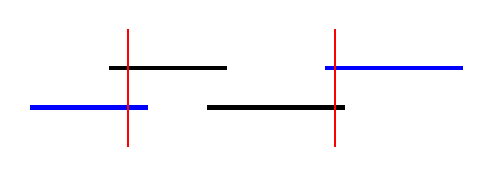
\begin{tikzpicture}
      \draw[blue, ultra thick] (0, 0) -- (1.5, 0);
      \draw[ultra thick] (1, .5) -- (2.5, .5);
      \draw[ultra thick] (2.25, 0) -- (4, 0);
      \draw[blue, ultra thick] (3.75, .5) -- (5.5, .5);
      \draw[red, thick] (1.25, -.5) -- (1.25, 1);
      \draw[red, thick] (3.875, -.5) -- (3.875, 1);
    \end{tikzpicture}
    \caption{$\nu(\mathcal F) = \tau(\mathcal F) = 2$.}
  \end{subfigure}
  \hfill
  \begin{subfigure}[b]{0.45\textwidth}
    \centering
    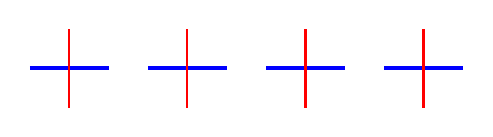
\begin{tikzpicture}
      \draw[blue, ultra thick] (0, 0) -- (1, 0);
      \draw[blue, ultra thick] (1.5, 0) -- (2.5, 0);
      \draw[blue, ultra thick] (3, 0) -- (4, 0);
      \draw[blue, ultra thick] (4.5, 0) -- (5.5, 0);
      \draw[red, thick] (.5, -.5) -- (.5, .5);
      \draw[red, thick] (2, -.5) -- (2, .5);
      \draw[red, thick] (3.5, -.5) -- (3.5, .5);
      \draw[red, thick] (5, -.5) -- (5, .5);
    \end{tikzpicture}
    \caption{$\nu(\mathcal F) = \tau(\mathcal F) = 4$.}
  \end{subfigure}
  \caption{Two examples of the matching number and the covering number of a finite family of compact intervals in $\RR$, where red vertical lines denote a minimum set of points that intersect all intervals in $\mathcal F$, and blue intervals denote a maximum set of pairwise disjoint intervals.}
  \label{fig:nu-tau}
\end{figure}

\begin{theorem}[Gallai, 1960]
  If $\mathcal F$ is a finite family of compact intervals in $\RR$, then $\tau(\mathcal F) = \nu(\mathcal F)$.
\end{theorem}

It is trivial to see that $\tau(\mathcal F) \geq \nu(\mathcal F)$, as any set of $k$ pairwise disjoint intervals requires $k$ points to intersect all the intervals in the set. We reformulate Gallai's theorem as follows:

\begin{theorem}[Gallai, 1960]
  Let $\mathcal F$ be a finite family of compact intervals in $\RR$. If $\tau(\mathcal F) > k$, then there exists a matching in $\mathcal F$ of size $k + 1$.
\end{theorem}

We consider the following colorful version of Gallai's theorem:

\begin{problem}
  Let $\mathcal F_1, \ldots, \mathcal F_{k + 1}$ be $k + 1$ families of intervals in $\RR$ such that $\tau(\mathcal F_i) > k$ for all $i \in [k + 1]$. Can one find a \emph{rainbow matching}, where a \emph{rainbow matching} is a matching $\mathcal M$ such that $|\mathcal M \cap \mathcal F_i| = 1$ for all $i \in [k + 1]$?
\end{problem}

Figure \ref{fig:colorful-gallai} gives an example of the colorful version of Gallai's theorem.

\begin{figure}[h]
  \centering
  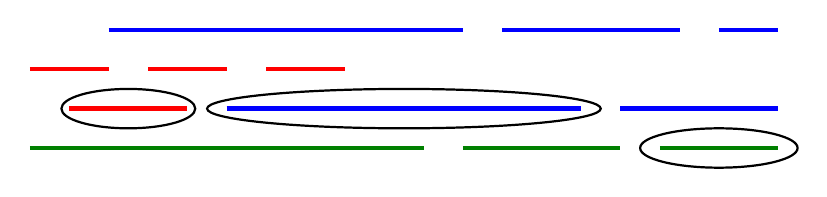
\begin{tikzpicture}
    \draw[Green, ultra thick] (0, 0) -- (5, 0);
    \draw[Green, ultra thick] (5.5, 0) -- (7.5, 0);
    \draw[Green, ultra thick] (8, 0) -- (9.5, 0);
    \draw[red, ultra thick] (0, 1) -- (1, 1);
    \draw[red, ultra thick] (1.5, 1) -- (2.5, 1);
    \draw[red, ultra thick] (3, 1) -- (4, 1);
    \draw[red, ultra thick] (.5, .5) -- (2, .5);
    \draw[blue, ultra thick] (2.5, .5) -- (7, .5);
    \draw[blue, ultra thick] (7.5, .5) -- (9.5, .5);
    \draw[blue, ultra thick] (1, 1.5) -- (5.5, 1.5);
    \draw[blue, ultra thick] (6, 1.5) -- (8.25, 1.5);
    \draw[blue, ultra thick] (8.75, 1.5) -- (9.5, 1.5);
    \draw[thick] (1.25, .5) ellipse (.85 and .25);
    \draw[thick] (4.75, .5) ellipse (2.5 and .25);
    \draw[thick] (8.75, 0) ellipse (1 and .25);
  \end{tikzpicture}
  \caption{An example of the colorful Gallai's theorem, where each family is denoted by a distinct color, the covering number of each family is greater than $2$, and a rainbow matching is circled.}
  \label{fig:colorful-gallai}
\end{figure}

\subsection{Fair Division of a Cake}

Consider a cake identified by $[0, 1]$ and $n$ players. Given any partition of the cake, each player gives a list of pieces they prefer in that partition. We say that a player is \emph{hungry} if they prefer a piece of positive length in any partition. Figure \ref{fig:empty} gives a partition of the cake with an empty piece.

\begin{figure}[h]
  \centering
  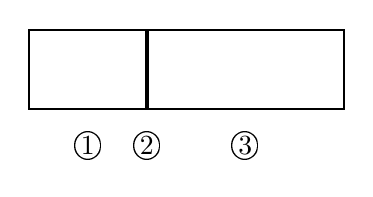
\begin{tikzpicture}
    \draw[thick] (0, 0) -- (4, 0) -- (4, 1) -- (0, 1) -- cycle;
    \draw[ultra thick] (1.5, 0) -- (1.5, 1);
    \node at (.75, -.5) {\textcircled{\raisebox{-1pt}{1}}};
    \node at (1.5, -.5) {\textcircled{\raisebox{-1pt}{2}}};
    \node at (2.75, -.5) {\textcircled{\raisebox{-1pt}{3}}};
  \end{tikzpicture}
  \caption{A partition of the cake, where the second piece is an empty piece.}
  \label{fig:empty}
\end{figure}

We say that a preference list is \emph{closed} if the following holds: if the player refers piece $i$ in a converging sequence of partitions, then they prefer piece $i$ also in the limiting partition. See Figure \ref{fig:closed} for an illustration.

\begin{figure}[h]
  \centering
  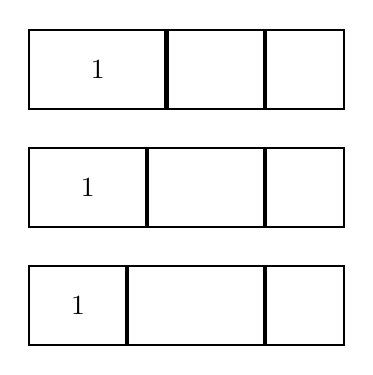
\begin{tikzpicture}
    \draw[thick] (0, 3) -- (4, 3) -- (4, 4) -- (0, 4) -- cycle;
    \draw[ultra thick] (1.75, 3) -- (1.75, 4);
    \draw[ultra thick] (3, 3) -- (3, 4);
    \draw[thick] (0, 1.5) -- (4, 1.5) -- (4, 2.5) -- (0, 2.5) -- cycle;
    \draw[ultra thick] (1.5, 1.5) -- (1.5, 2.5);
    \draw[ultra thick] (3, 1.5) -- (3, 2.5);
    \draw[thick] (0, 0) -- (4, 0) -- (4, 1) -- (0, 1) -- cycle;
    \draw[ultra thick] (1.25, 0) -- (1.25, 1);
    \draw[ultra thick] (3, 0) -- (3, 1);
    \node at (.875, 3.5) {$1$};
    \node at (.75, 2) {$1$};
    \node at (.625, .5) {$1$};
  \end{tikzpicture}
  \caption{Illustrating the concept of a closed preference list, where the three partitions indicate a converging sequence of partitions. If the first player prefers the first piece in every partition in this sequence, then they must prefer the first piece in the limiting partition.}
  \label{fig:closed}
\end{figure}

Moreover, we say that a division (i.e., a partition) is \emph{envy-free} if each player has a distinct piece in their preference list.

\begin{theorem}[Su, 1980]
  If every player is hungry, and if the preference list of each player is closed, then an envy-free division exists.
\end{theorem}

\end{document}
